\documentclass{standalone}
\usepackage{tikz}
\usepackage{ctex,siunitx}
\usepackage{tkz-euclide}
\usepackage{amsmath}
\usetikzlibrary{patterns, calc}
\usetikzlibrary {decorations.pathmorphing, decorations.pathreplacing, decorations.shapes,}
\begin{document}
\small
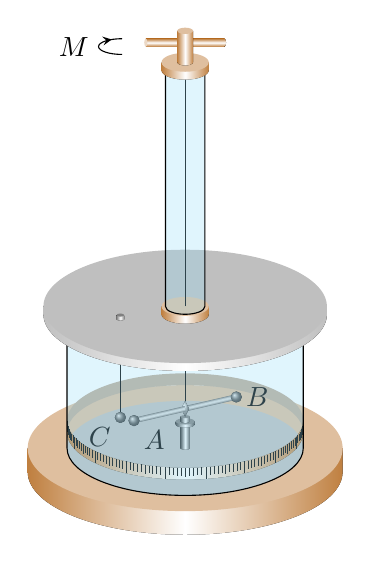
\begin{tikzpicture}[>=latex,scale=1]
  % \useasboundingbox(-1,-2)rectangle(8,6);
  \fill[left color=brown,right color=brown,middle color=white](-2,0.3)--(-2,0)arc(-180:0:2 and 0.8)--(2,0.3);
  \fill[brown!50](0,0.3)ellipse(2 and 0.8);
  \fill[lightgray](0,0.3)ellipse(1.5 and 0.6);
  \fill[left color=darkgray,right color=darkgray,middle color=white](0,0.3)ellipse(0.06 and 0.02);
  \fill[left color=darkgray,right color=darkgray,middle color=white](-0.06,0.3)rectangle(0.06,0.6);
  \fill[left color=darkgray,right color=darkgray,middle color=white](0,0.6)ellipse(0.12 and 0.04);
  \fill[left color=darkgray,right color=darkgray,middle color=white](-0.12,0.6)rectangle(0.12,0.64);
  \fill[gray](0,0.64)ellipse(0.12 and 0.04);
  \fill[left color=darkgray,right color=darkgray,middle color=white](0,0.64)ellipse(0.06 and 0.02);
  \fill[left color=darkgray,right color=darkgray,middle color=white](-0.06,0.64)rectangle(0.06,0.7);
  \fill[gray](0,0.7)ellipse(0.06 and 0.02);
  \fill[brown!30!lightgray](-1.5,0.65)--(-1.5,0.5)arc(180:0:1.5 and 0.6)--(1.5,0.65)arc(0:180:1.5 and 0.6);
  \draw(0,0.8)--++({0.75*cos(30)},{0.3*sin(30)}) coordinate (B);
  \foreach \w in {80,60,40,20} {\draw[darkgray!\w,line width={2*sin(\w)}](0,0.8)--++({0.75*cos(30)},{0.3*sin(30)});}
  \draw(0,0.8)--++({0.75*cos(210)},{0.3*sin(210)}) coordinate (A);
  \fill[ball color=gray](B) circle(2pt) node[right]{$B$};
  \fill[ball color=lightgray](0,0.7)--(0.05,0.8)--(0,0.9)--(-0.05,0.8)--cycle;
  \foreach \w in {80,60,40,20} {\draw[darkgray!\w,line width={2*sin(\w)}](0,0.8)--++({0.75*cos(210)},{0.3*sin(210)});}
  \fill[ball color=gray](A) circle(2pt)node[below right]{$A$};
  \draw(A)++({0.2*cos(150)},{0.08*sin(150)}) coordinate (C);
  \coordinate(D) at (C|-0,2.0);
  \draw[very thin](C)--(D)(0,0.9)--(0,2.0);
  \fill[ball color=gray](C) circle(2pt)node[below left]{$C$};
  \fill[left color=brown,right color=brown,middle color=white](-1.5,0.65)--(-1.5,0.5)arc(-180:0:1.5 and 0.6)--(1.5,0.65)arc(0:-180:1.5 and 0.6);
  \foreach \x in {-180,-160,...,-20}
  {
    \draw[ultra thin]({1.5*cos(\x)},{0.65+0.6*sin(\x)})--++(0,-0.15);
    \draw[ultra thin]({1.5*cos(\x+10)},{0.65+0.6*sin(\x+10)})--++(0,-0.12);
    \foreach \y in {2,4,6,8,12,14,16,18}
    {
      \draw[ultra thin]({1.5*cos(\x+\y)},{0.65+0.6*sin(\x+\y)})--++(0,-0.1);
    }
  }
  \draw[ultra thin](1.5,0.5)--++(0,0.15);
  \draw[fill=cyan!40,fill opacity=0.3](-1.5,2.0)--(-1.5,0.3)arc(-180:0:1.5 and 0.6)--(1.5,2.0)--cycle;
  \fill[left color=lightgray,right color=lightgray,middle color=white](0,2.0)ellipse(1.8 and 0.72);
  \fill[left color=lightgray,right color=lightgray,middle color=white](-1.8,2.0)rectangle(1.8,2.1);
  \fill[lightgray](0,2.1)ellipse(1.8 and 0.72);
  \fill[left color=gray,right color=gray,middle color=white]([yshift=-0.6mm]D)ellipse(0.05 and 0.02);
  \fill[left color=gray,right color=gray,middle color=white]([xshift=-0.5mm,yshift=-0.6mm]D)rectangle++(0.1,0.05);
  \fill[gray]([yshift=-0.1mm]D)ellipse(0.05 and 0.02);
  \fill[left color=brown,right color=brown,middle color=white](-0.3,2.1)--(-.3,2.0)arc(-180:0:0.3 and 0.12)--(0.3,2.1);
  \fill[brown!50](0,2.1)ellipse(0.3 and 0.12);
  \draw[very thin](0,2.1)--(0,5.1);
  \draw[fill=cyan!40,fill opacity=0.3](-0.25,5.1)--(-0.25,2.1)arc(-180:0:0.25 and 0.1)--(0.25,5.1)--cycle;
  \fill[left color=brown,right color=brown,middle color=white](-0.3,5.2)--(-.3,5.1)arc(-180:0:0.3 and 0.12)--(0.3,5.2);
  \fill[brown!50](0,5.2)ellipse(0.3 and 0.12);
  \fill[top color=brown,bottom color=brown,middle color=white](0.5,5.45)ellipse(0.02 and 0.05);
  \fill[top color=brown,bottom color=brown,middle color=white](-0.5,5.4)rectangle(0.5,5.5);
  \fill[brown!30](-0.5,5.45)ellipse(0.02 and 0.05);
  \fill[left color=brown,right color=brown,middle color=white](-0.1,5.6)--(-.1,5.2)arc(-180:0:0.1 and 0.04)--(0.1,5.6);
  \fill[brown!50](0,5.6)ellipse(0.1 and 0.04);
  \draw[thin,postaction={decorate},decoration={markings,mark=at position 0.2 with {\arrowreversed{stealth}}}](-0.8,5.5)arc(90:270:0.3 and 0.1)node[midway,left]{$M$};
\end{tikzpicture}
\end{document}